\section{Background}\label{sec:background}
% General introduction
The exponential tendency for data demand to the \textit{zettabyte} era, predicted by major network providers \cite{cisco2016forecast,kremling2015presentation,belllabs2016report,ericsson2015report}, is present and evident. The use of cellular networks for data consumption has become a widespread topic to the general audience. The reason has been the flourishement of online applications services from the last two decades such as:  Whatsapp, Viber (voice and messaging), Facebook, Twitter, Snapchat, Instagram, Google+ (social networking), YouTube, Netflix, SoundCloud, Spotify (video or audio streaming), Google Drive, Dropbox and OneDrive (data storage). Also, these applications have been developed not only for a \ac{PC} but also mobile smartphones, tablets and phablets that support either the Android, iOS or Windows Mobile \ac{OS}. Further, content delivery networks will be carrying two-thirds of the Internet traffic by the end of 2016 \cite{cisco2016forecast}. Hence, it is expected that the data growth will continue within this market. From all these services, streaming applications that are based in multicast scenarios where a transmitter needs to serve tens, hundreds or even thousands of receivers are becoming more frequent in mobile networks such as \ac{LTE-A} or \ac{WLAN} networks such as \ac{WiFi}. These types of scenarios pose tight requirements in terms of data throughput and delay to ensure a satisfactoring \ac{QoE}.

For the network operator, techniques that can offload the service infrastructure to cope with such data load are needed in order to satisfy the increasing demand. Further, due to network capacity constraints, the end-user might not be connected to a \ac{BS} in a cellular fashion. Instead, the connectivity might be provided by other users either within the cellular spectrum or through a \ac{WLAN}. The deployment of mobile devices without cellular coverage but in a local network can potentially be decentralized. This type of deployment will require the communicating devices to (i) employ multihop communications to ensure connectivity, (ii) use control access mechanisms to avoid interference in the local network. From the devices perspective, energy consumption due to data transmissions has become a limiting factor in terms of battery life. The reason is that mobile devices perform much more internal tasks than older devices from ten years ago. Therefore, mobile network designers need to consider mechanisms and techniques that aim for high throughput and low energy consumption both at the station and the end user devices and that are able to provide data offloading from current network infrastructures.

\subsection{Network Coding for Cooperative Wireless Networks}
% Cooperation
The concept of cooperation in wireless networks has been investigated before \cite{fitzek2006cooperation,fitzek2007cognitive,heide2012green,fitzek2013implementation,fitzek2013mobile}. The main goal is to diminish the amount of communications resources (data rate, energy or even storage and computational power) to convey an information of common interest from a transmitter to a set of interconnected receivers in a multicast fashion. Devices connected in this way form a \textit{mobile cloud} \cite{fitzek2013mobile}. In Fig.~\ref{fig:cooperation}, it can be observed a comparison example of no cooperation and cooperation in a multicast wireless network.

\begin{figure}[ht!]
  \centering 
  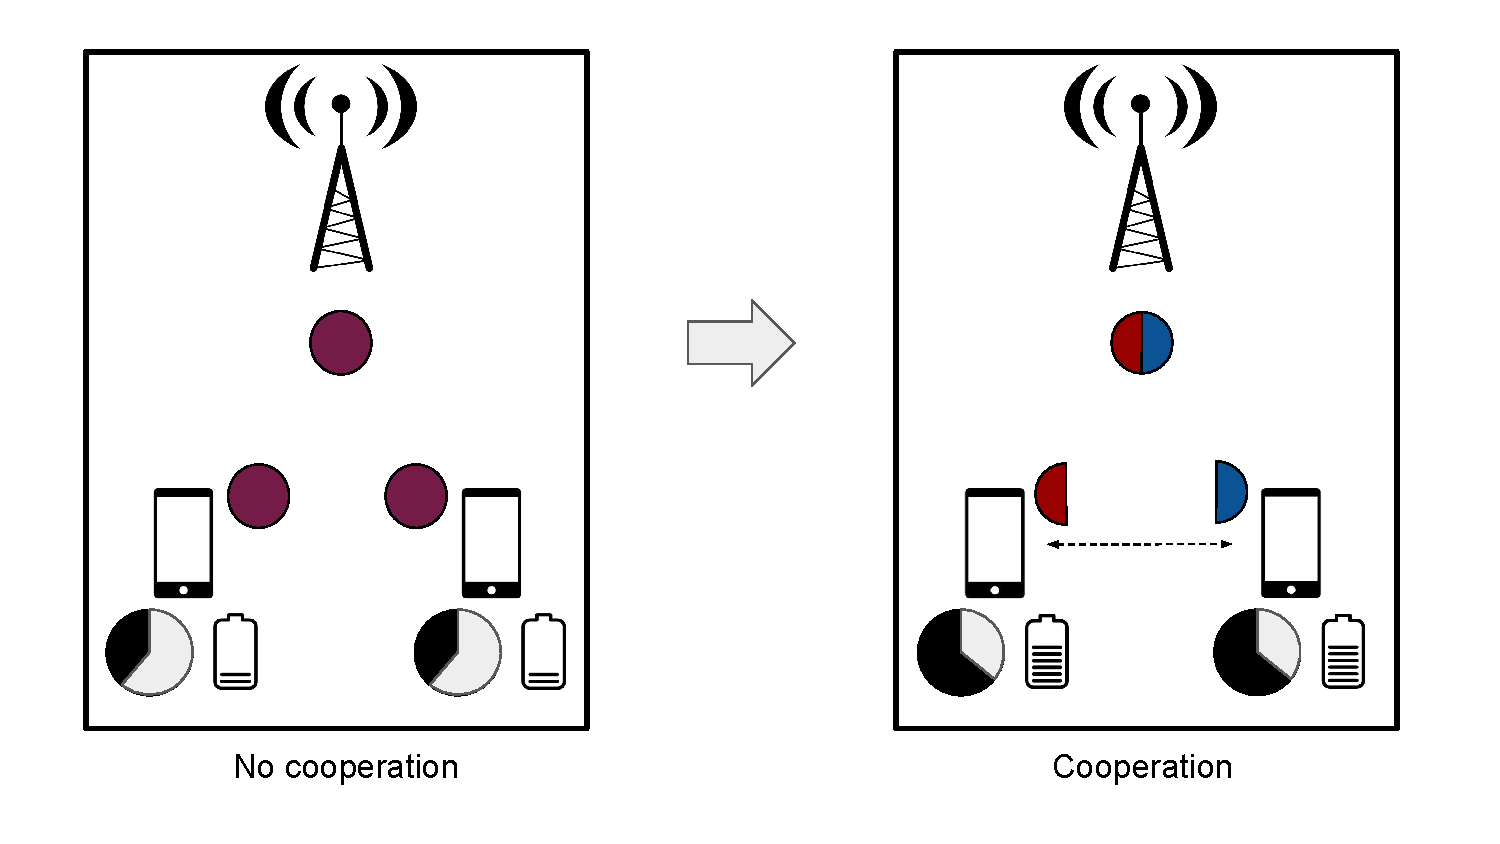
\includegraphics[width=\textwidth]{introduction/figures/cooperation.pdf}
  \caption{Cooperation in Wireless Networks.}
\label{fig:cooperation}
\end{figure} 

Without cooperation, a purple content is sent to two mobile devices in a broadcast fashion. This incurs in posible a large downloading time to ensure both devices are satisfied reducing the throughput and increasing the energy consumption.  When cooperation is considered, the content now is split into smaller blue and red pieces where each of them is sent rapidly to each device. Then, the devices exploit short-range communications (dashed line) by exchanging their missing pieces. The key underlying idea is for the devices share their missing information through a faster, short-distance and reliable link which increases the total throughput and reduces the overal energy consumption. From an operator perspective, the information \textit{as a whole} is quickly disseminated into the receivers helping the \ac{BS} to offload data. At the end, the goal of making the cluster share resources is achieved. In this way, mobile clouds allow to improve the overall network performance and user experience.

One of the key aspects to achieve the gains proposed by the cooperative approach is the short-range technologies to be considered. Besides \ac{WLAN} technologies such as Bluetooth or \ac{WiFi}, there has been a large interest in \ac{D2D} communications. These type of communications allows the devices to share data without going through the cellular network which keeps the idea of data offloading. In \ac{LTE-A} networks, \ac{D2D} applications services have been included \cite{3gpp2012prose} to evaluate its improvements in the \ac{QoE}.

% Network Coding, RLNC and applications
Introduced by Alshwede et al. \cite{ahlswede2000network}, \ac{NC} appeared as an effective technology to remove the limitations presented previously. In this work, the authors presented a new paradigm for conveying information in communication networks. Instead of following the convention of forwarding data packets from two different data flows, the packets are mixed to create new coded packets. To decode, by receiving a coded packet and knowing the original packets, it is possible to extract the missing information. This key idea let the research community know for the first time that it was possible to code on a \textit{network} basis and not only on a \textit{link} basis as conventional \ac{FEC} technologies do. In the State-of-the-Art, mainly two types of network coding can be identified according to how the packets are mixed from: inter-session network coding and intra session network coding. 

\subsection{Thesis Objectives}
Describe the objectives here from Fig.~\ref{fig:proposal}.

\begin{figure}[ht!]
  \centering 
  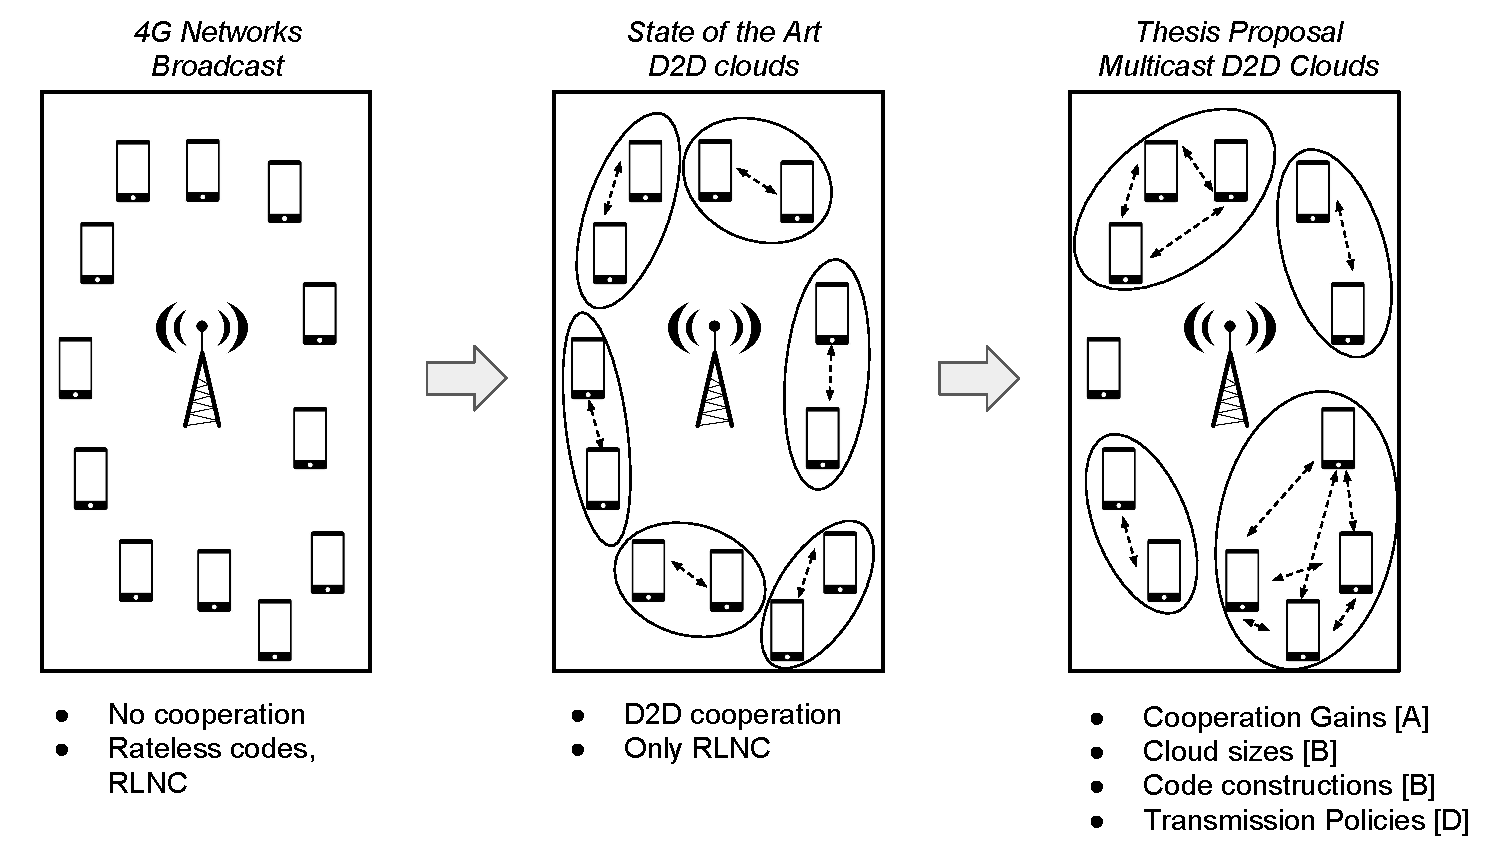
\includegraphics[width=\textwidth]{introduction/figures/thesis-diagrams.pdf}
  \caption{State of the Art and Thesis Proposal.}
\label{fig:proposal}
\end{figure} 
